\question An insulating ring of radius $R$ is arranged such that one half has charge $+Q$ uniformly distributed and another half has charge $-Q$ uniformly distributed. What is the electric field vector $\efield$ at the center of the ring?

\begin{center}
	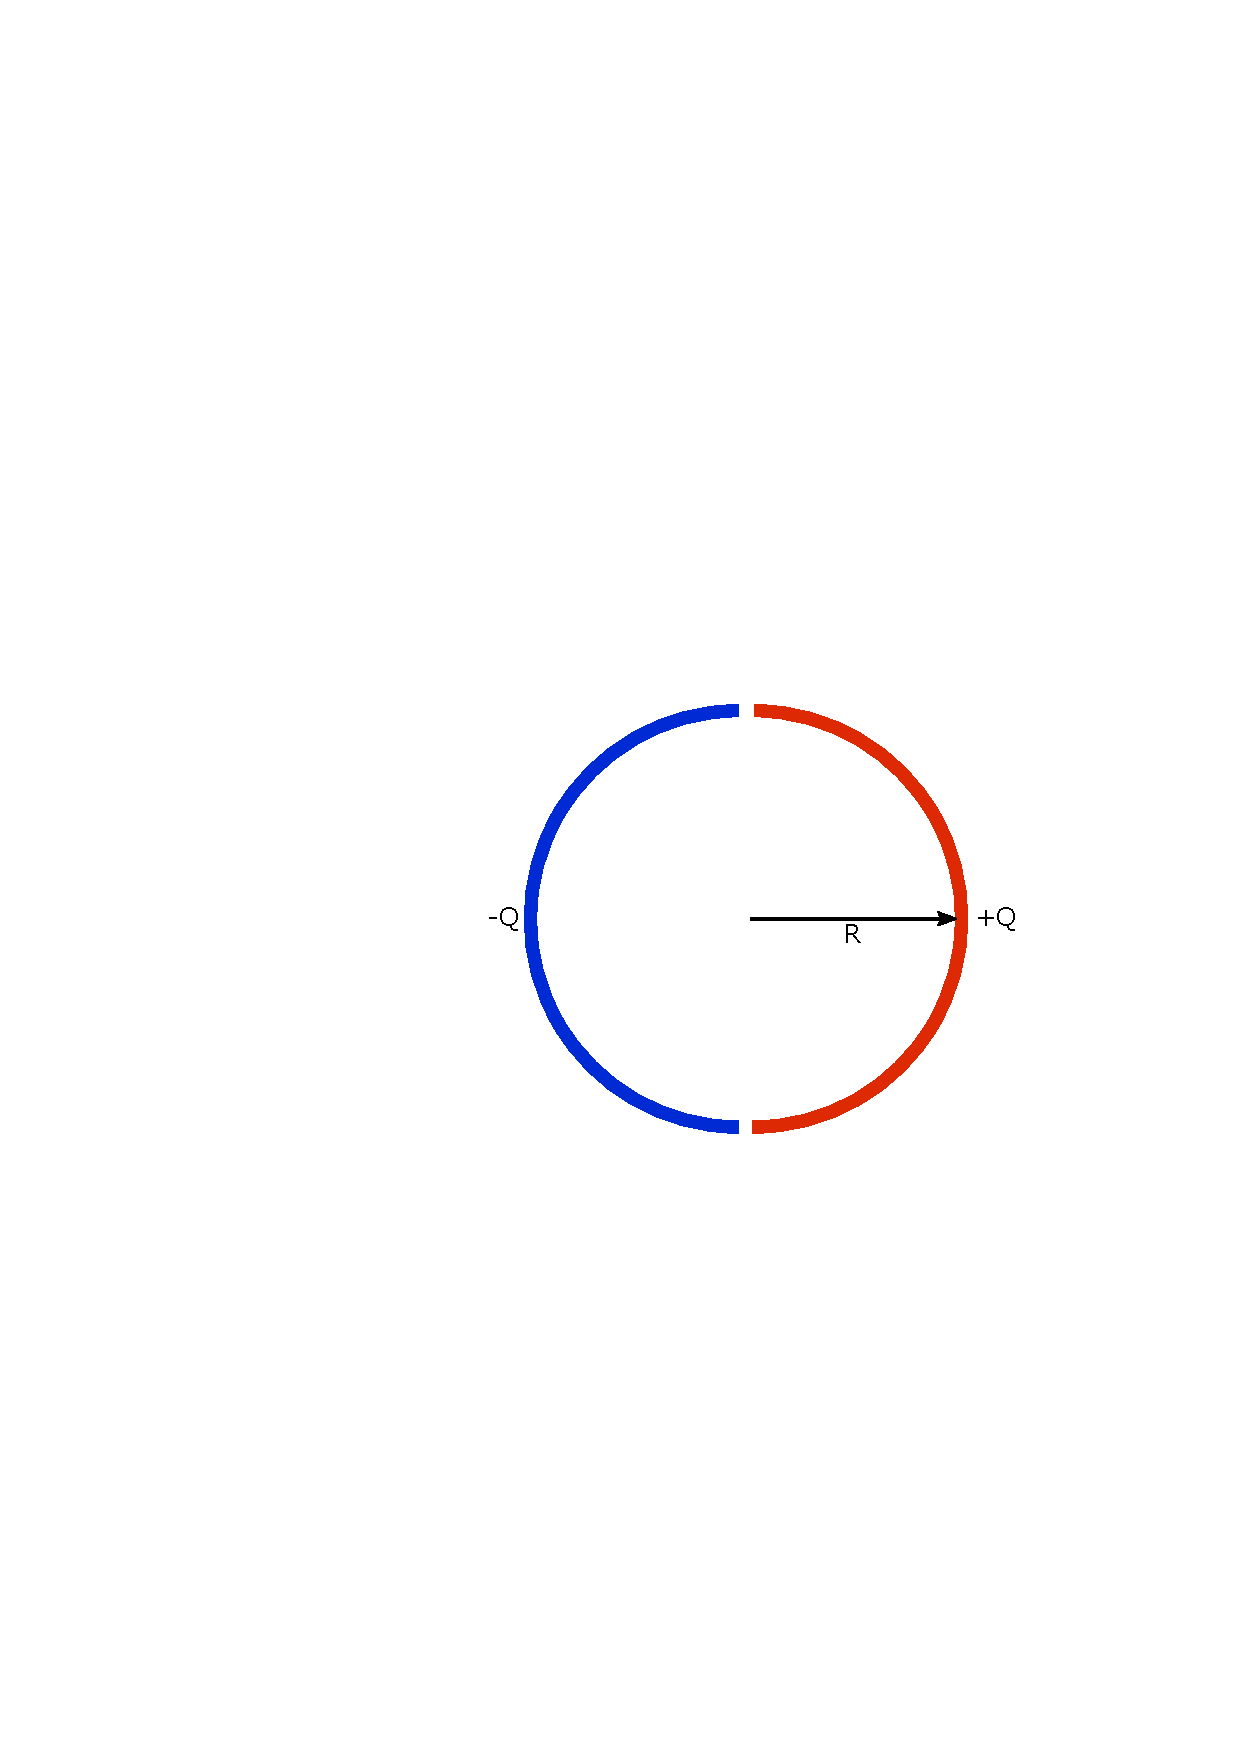
\includegraphics[width=8cm]{prob5.pdf}
\end{center}